\documentclass[11pt,a4paper]{report}
\usepackage[textwidth=37em,vmargin=30mm]{geometry}
\usepackage{calc,xunicode,amsmath,amssymb,paralist,enumitem,tabu,booktabs,datetime2,xeCJK,xeCJKfntef,listings}
\usepackage{tocloft,fancyhdr,tcolorbox,xcolor,graphicx,eso-pic,xltxtra,xelatexemoji}

\newcommand{\envyear}[0]{2025}
\newcommand{\envdatestr}[0]{2025-10-26}
\newcommand{\envfinaldir}[0]{webdb/2025/20251026/final}

\usepackage[hidelinks]{hyperref}
\hypersetup{
    colorlinks=false,
    pdfpagemode=FullScreen,
    pdftitle={Web Digest - \envdatestr}
}

\setlength{\cftbeforechapskip}{10pt}
\renewcommand{\cftchapfont}{\rmfamily\bfseries\large\raggedright}
\setlength{\cftbeforesecskip}{2pt}
\renewcommand{\cftsecfont}{\sffamily\small\raggedright}

\setdefaultleftmargin{2em}{2em}{1em}{1em}{1em}{1em}

\usepackage{xeCJK,xeCJKfntef}
\xeCJKsetup{PunctStyle=plain,RubberPunctSkip=false,CJKglue=\strut\hskip 0pt plus 0.1em minus 0.05em,CJKecglue=\strut\hskip 0.22em plus 0.2em}
\XeTeXlinebreaklocale "zh"
\XeTeXlinebreakskip = 0pt


\setmainfont{Brygada 1918}
\setromanfont{Brygada 1918}
\setsansfont{IBM Plex Sans}
\setmonofont{JetBrains Mono NL}
\setCJKmainfont{Noto Serif CJK SC}
\setCJKromanfont{Noto Serif CJK SC}
\setCJKsansfont{Noto Sans CJK SC}
\setCJKmonofont{Noto Sans CJK SC}

\setlength{\parindent}{0pt}
\setlength{\parskip}{8pt}
\linespread{1.15}

\lstset{
	basicstyle=\ttfamily\footnotesize,
	numbersep=5pt,
	backgroundcolor=\color{black!5},
	showspaces=false,
	showstringspaces=false,
	showtabs=false,
	tabsize=2,
	captionpos=b,
	breaklines=true,
	breakatwhitespace=true,
	breakautoindent=true,
	linewidth=\textwidth
}






\newcommand{\coverpic}[2]{
    % argv: itemurl, authorname
    Cover photo by #2~~(\href{#1}{#1})
}
\newcommand{\makeheader}[0]{
    \begin{titlepage}
        % \newgeometry{hmargin=15mm,tmargin=21mm,bmargin=12mm}
        \begin{center}
            
            \rmfamily\scshape
            \fontspec{BaskervilleF}
            \fontspec{Old Standard}
            \fontsize{59pt}{70pt}\selectfont
            WEB\hfill DIGEST
            
            \vfill
            % \vskip 30pt
            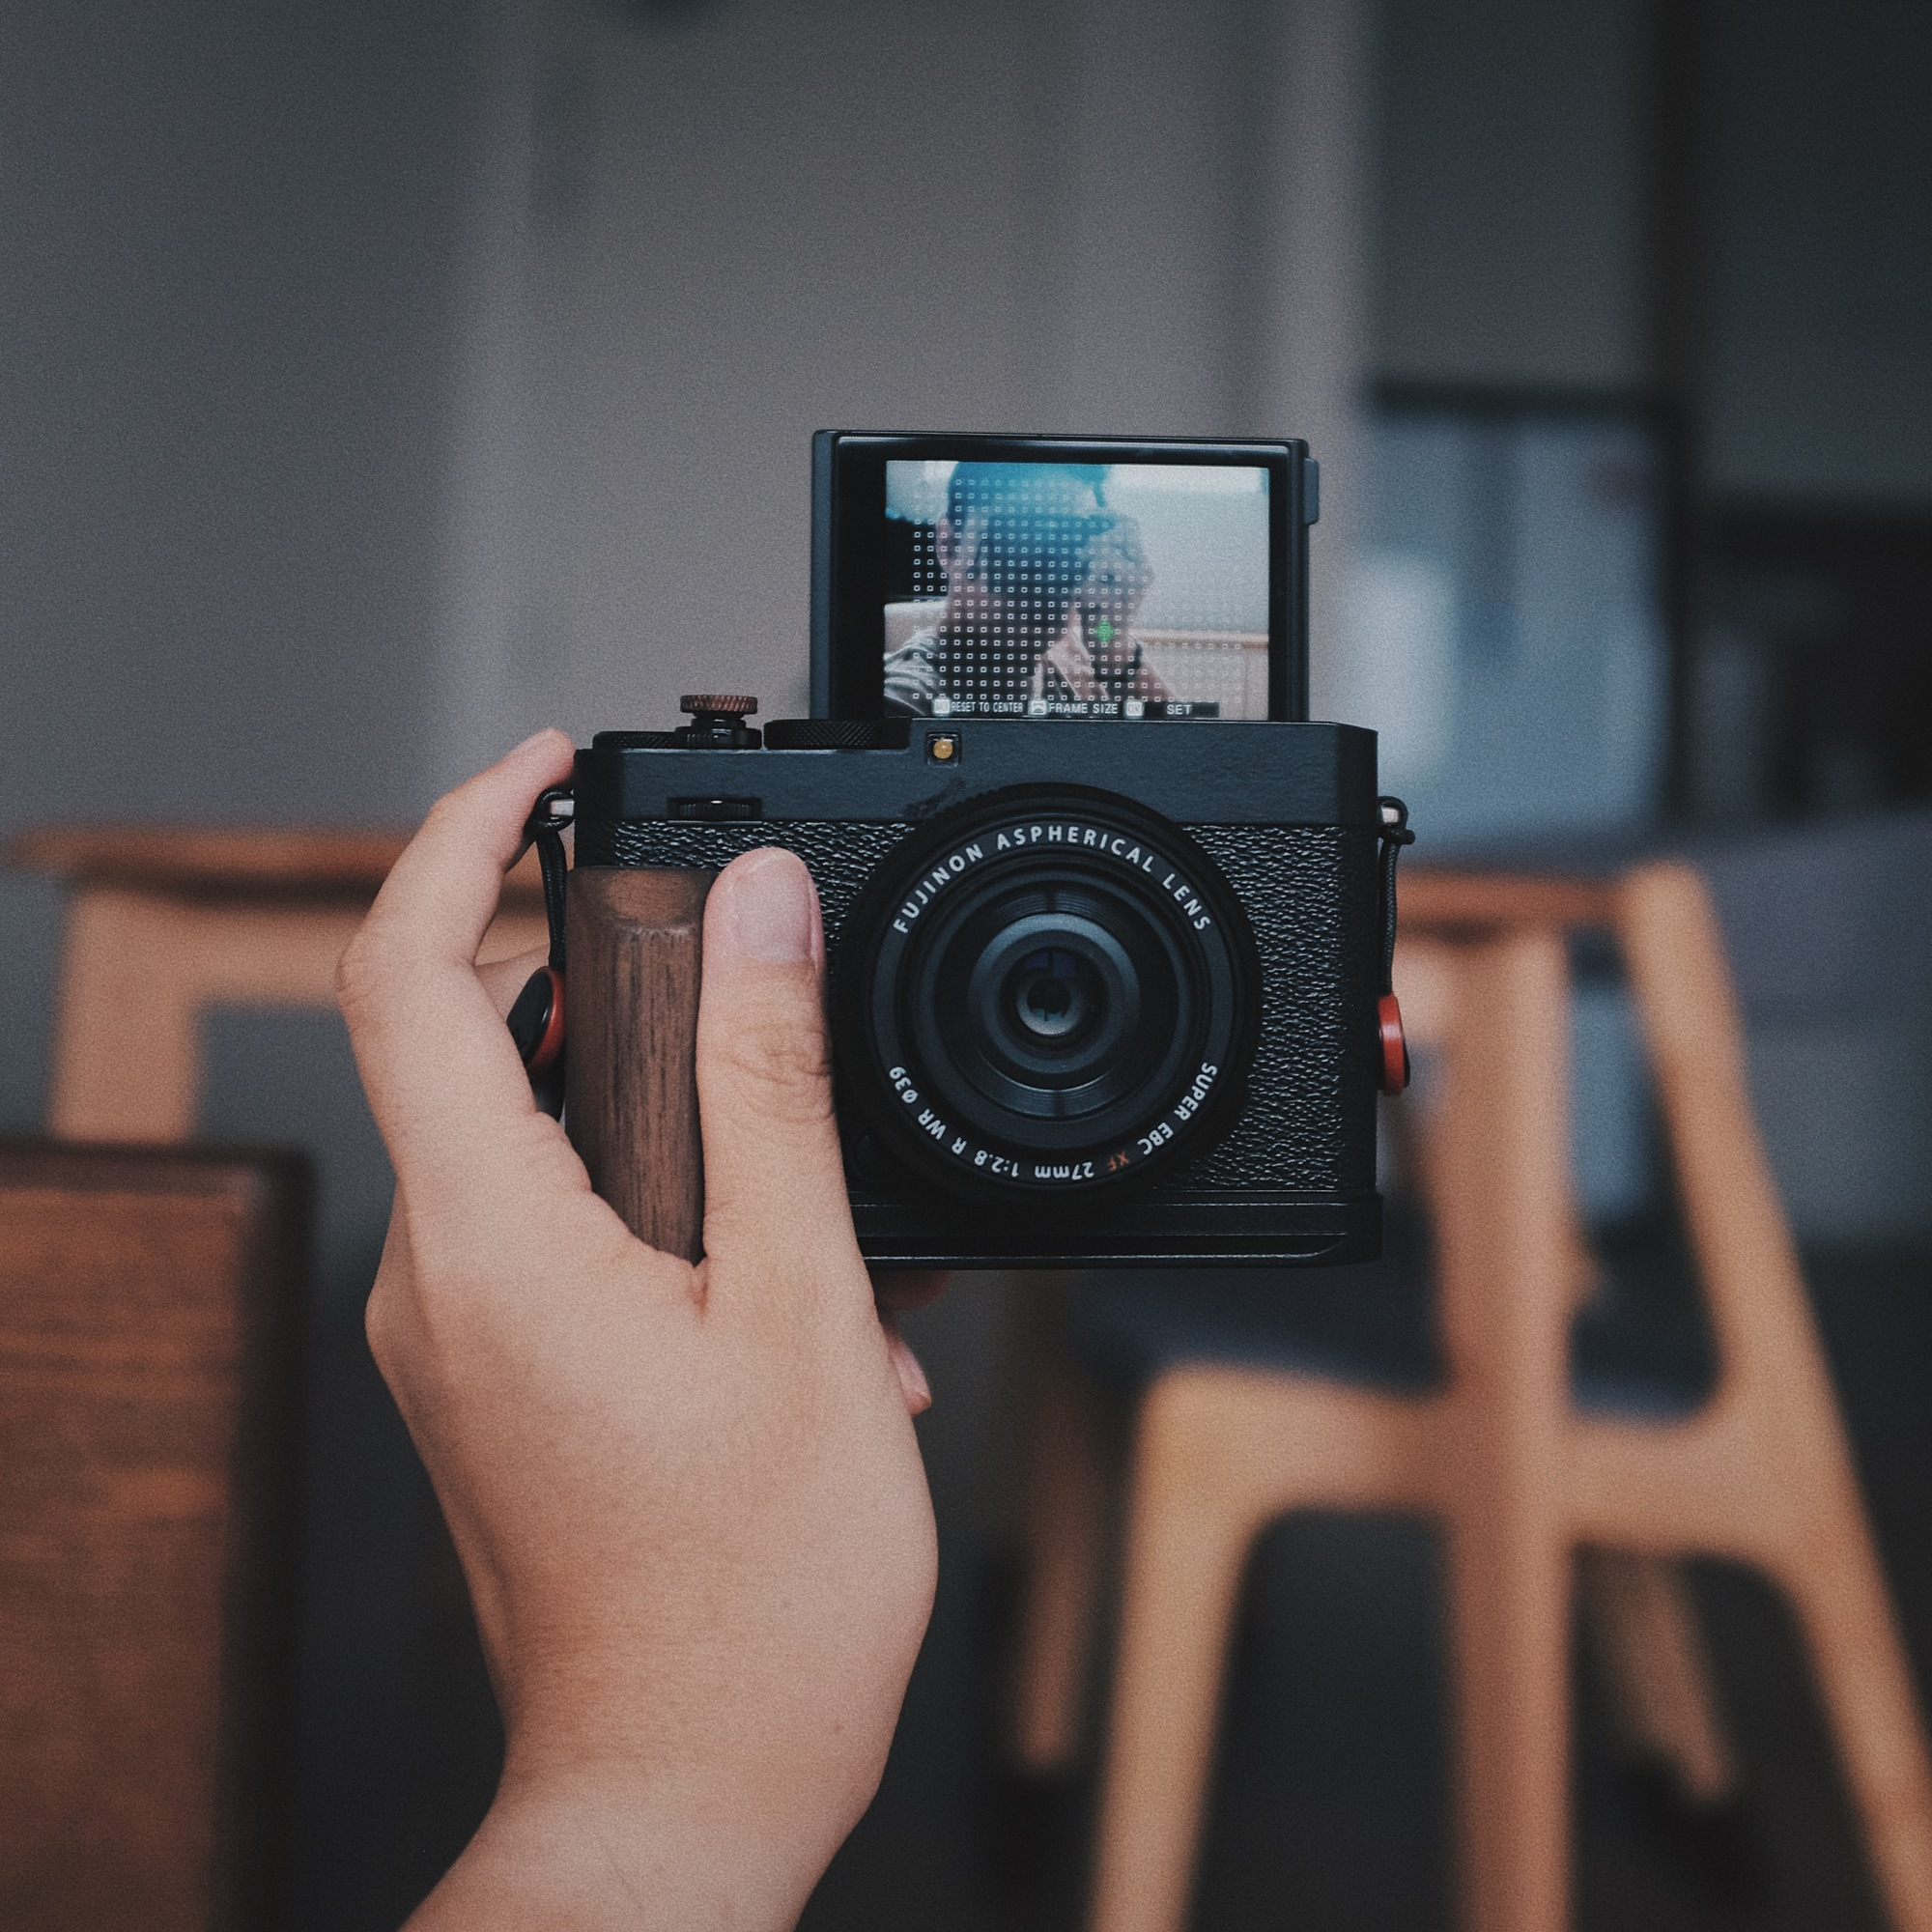
\includegraphics[width=\linewidth]{\envfinaldir/coverpic-prod.jpg}\par
            % \vskip 30pt
            \vfill

            \normalsize\rmfamily\scshape
            \copyright{} The Web Digest Project \hfill\large \envdatestr
        \end{center}
    \end{titlepage}
    % \restoregeometry
}
\newcommand{\simplehref}[1]{%
    \textcolor{blue!80!green}{\href{#1}{#1}}%
}
\renewcommand{\contentsname}{\center\Huge\sffamily\bfseries Contents\par\vskip 20pt}
\newcounter{ipartcounter}
\setcounter{ipartcounter}{0}
\newcommand{\ipart}[1]{
    % \vskip 20pt
    \clearpage
    \stepcounter{ipartcounter}
    \phantomsection
    \addcontentsline{toc}{chapter}{#1}
    % \begin{center}
    %     \Huge
    %     \sffamily\bfseries
    %     #1
    % \end{center}
    % \vskip 20pt plus 7pt
}
\newcounter{ichaptercounter}
\setcounter{ichaptercounter}{0}
\newcommand{\ichapter}[1]{
    % \vskip 20pt
    \clearpage
    \stepcounter{ichaptercounter}
    \phantomsection
    \addcontentsline{toc}{section}{\numberline{\arabic{ichaptercounter}}#1}
    \begin{center}
        \Huge
        \sffamily\bfseries
        #1
    \end{center}
    \vskip 20pt plus 7pt
}
\newcommand{\entrytitlefont}[1]{\subsection*{\raggedright\Large\sffamily\bfseries#1}}
\newcommand{\entryitemGeneric}[2]{
    % argv: title, url
    \parbox{\linewidth}{
        \entrytitlefont{#1}\par\vskip 5pt
        \footnotesize\ttfamily\mdseries
        \simplehref{#2}
    }\vskip 11pt plus 11pt minus 1pt
}
\newcommand{\entryitemGithub}[3]{
    % argv: title, url, desc
    \parbox{\linewidth}{
        \entrytitlefont{#1}\par\vskip 5pt
        \footnotesize\ttfamily\mdseries
        \simplehref{#2}\par\vskip 5pt
        \small\rmfamily\mdseries#3
    }\vskip 11pt plus 11pt minus 1pt
}
\newcommand{\entryitemAp}[3]{
    % argv: title, url, desc
    \parbox{\linewidth}{
        \entrytitlefont{#1}\par\vskip 5pt
        \footnotesize\ttfamily\mdseries
        \simplehref{#2}\par\vskip 5pt
        \small\rmfamily\mdseries#3
    }\vskip 11pt plus 11pt minus 1pt
}
\newcommand{\entryitemHackernews}[3]{
    % argv: title, hnurl, rawurl
    % \parbox{\linewidth}{
    %     \entrytitlefont{#1}\par\vskip 5pt
    %     \footnotesize\ttfamily\mdseries
    %     \simplehref{#3}\par
    %     \textcolor{black!50}{\href{#2}{#2}}
    % }\vskip 11pt plus 11pt minus 1pt
    \begin{minipage}{\linewidth}
            \entrytitlefont{#1}\par\vskip 5pt
            \footnotesize\ttfamily\mdseries
            \simplehref{#3}\par
            \textcolor{black!50}{\href{#2}{#2}}
    \end{minipage}\par\vskip 11pt plus 11pt minus 1pt
}







\begin{document}

\makeheader

\tableofcontents\clearpage




\ipart{Developers}
\ichapter{Hacker News}
\entryitemTwoLinks{California invests in battery energy storage, leaving rolling blackouts behind}{https://news.ycombinator.com/item?id=45706527}{https://www.latimes.com/environment/story/2025-10-17/california-made-it-through-another-summer-without-a-flex-alert}

\entryitemTwoLinks{The Journey Before main()}{https://news.ycombinator.com/item?id=45706380}{https://amit.prasad.me/blog/before-main}

\entryitemTwoLinks{We do not have sufficient links to the UK for Online Safety Act to be applicable}{https://news.ycombinator.com/item?id=45705381}{https://libera.chat/news/advised}

\entryitemTwoLinks{Rock Tumbler Instructions}{https://news.ycombinator.com/item?id=45705125}{https://rocktumbler.com/tips/rock-tumbler-instructions/}

\entryitemTwoLinks{Windows 10 Deadline Boosts Mac Sales}{https://news.ycombinator.com/item?id=45704616}{https://www.macrumors.com/2025/10/25/windows-10-deadline-boosts-mac-sales/}

\entryitemTwoLinks{Synadia and TigerBeetle Commit \$512k USD to the Zig Software Foundation}{https://news.ycombinator.com/item?id=45703716}{https://www.synadia.com/blog/synadia-tigerbeetle-zig-foundation-pledge}

\entryitemTwoLinks{Making a micro Linux distro (2023)}{https://news.ycombinator.com/item?id=45703556}{https://popovicu.com/posts/making-a-micro-linux-distro/}

\entryitemTwoLinks{React vs. Backbone in 2025}{https://news.ycombinator.com/item?id=45702558}{https://backbonenotbad.hyperclay.com/}

\entryitemTwoLinks{Tell HN: OpenAI now requires ID verification and won't refund API credits}{https://news.ycombinator.com/item?id=45702363}{https://news.ycombinator.com/item?id=45702363}

\entryitemTwoLinks{Euro cops take down cybercrime network with 49M fake accounts}{https://news.ycombinator.com/item?id=45701825}{https://www.itnews.com.au/news/euro-cops-take-down-cybercrime-network-with-49-million-fake-accounts-621174}

\entryitemTwoLinks{Meet the real screen addicts: the elderly}{https://news.ycombinator.com/item?id=45701305}{https://www.economist.com/international/2025/10/23/meet-the-real-screen-addicts-the-elderly}

\entryitemTwoLinks{Key IOCs for Pegasus and Predator Spyware Removed with iOS 26 Update}{https://news.ycombinator.com/item?id=45700946}{https://iverify.io/blog/key-iocs-for-pegasus-and-predator-spyware-cleaned-with-ios-26-update}

\entryitemTwoLinks{Advice for new principal tech ICs (i.e., notes to myself)}{https://news.ycombinator.com/item?id=45700911}{https://eugeneyan.com/writing/principal/}

\entryitemTwoLinks{What is intelligence? (2024)}{https://news.ycombinator.com/item?id=45700663}{https://whatisintelligence.antikythera.org/}

\entryitemTwoLinks{New OSM file format: 30\% smaller than PBF, 5x faster to import}{https://news.ycombinator.com/item?id=45699725}{https://community.openstreetmap.org/t/new-osm-file-format-30-smaller-than-pbf-5x-faster-to-import/137151}

\entryitemTwoLinks{Study: MRI contrast agent causes harmful metal buildup in some patients}{https://news.ycombinator.com/item?id=45698909}{https://www.ormanager.com/briefs/study-mri-contrast-agent-causes-harmful-metal-buildup-in-some-patients/}

\entryitemTwoLinks{The Swift SDK for Android}{https://news.ycombinator.com/item?id=45698570}{https://www.swift.org/blog/nightly-swift-sdk-for-android/}

\entryitemTwoLinks{Harnessing America's heat pump moment}{https://news.ycombinator.com/item?id=45698554}{https://www.heatpumped.org/p/harnessing-america-s-heat-pump-moment}

\entryitemTwoLinks{FBI Agents Visit Anti-ICE Protester: "Your name was brought up."}{https://news.ycombinator.com/item?id=45697395}{https://www.kenklippenstein.com/p/video-fbi-agents-visit-anti-ice-protester}

\entryitemTwoLinks{How to make a Smith chart}{https://news.ycombinator.com/item?id=45696838}{https://www.johndcook.com/blog/2025/10/23/smith-chart/}\ichapter{Phoronix}
\entryitemGeneric{\hskip 0pt{}Resources 1.9 Brings Intel Xe GPU Support \& Other System Resource Monitoring For GNOME}{https://www.phoronix.com/news/GNOME-Resources-1.9}

\entryitemGeneric{\hskip 0pt{}NVIDIA Starts Posting Open-Source Nova Driver Patches To Prep For Next-Gen GPUs}{https://www.phoronix.com/news/NVIDIA-Nova-Next-Gen-Boot42}

\entryitemGeneric{\hskip 0pt{}Servo's Demo Browser Adds Experimental Mode \& More Performance Improvements}{https://www.phoronix.com/news/Servo-September-2025-Highlights}

\entryitemGeneric{\hskip 0pt{}KDE Plasma 6.6 Will Cater To Windows Power Users With "winver"}{https://www.phoronix.com/news/KDE-Plasma-6.6-winver}

\entryitemGeneric{\hskip 0pt{}FreeBSD 15.0 Beta 3 Brings Working Support For MediaTek MT76 WiFi}{https://www.phoronix.com/news/FreeBSD-15.0-Beta-3}

\entryitemGeneric{\hskip 0pt{}Rust Coreutils 0.3 Released With Some Major Speed-Ups, Better GNU Compatibility}{https://www.phoronix.com/news/Rust-Coreutils-0.3-Released}

\entryitemGeneric{\hskip 0pt{}OpenGL Sees New Extensions Added To The Registry}{https://www.phoronix.com/news/OpenGL-October-2025-Extensions}

\entryitemGeneric{\hskip 0pt{}The Latest Sheaves Work To Hopefully Improve Linux Performance}{https://www.phoronix.com/news/Sheaves-Replace-CPU-Slabs}

\entryitemGeneric{\hskip 0pt{}Linux Lands Fix For "Serious Performance Regression" Affecting Some Intel Chromebooks}{https://www.phoronix.com/news/Linux-618-rc3-Fix-Chromebook-PM}


\ipart{Developers~~~~(zh-Hans)}
\ichapter{Solidot}
\entryitemGeneric{\hskip 0pt{}2023 年海洋热浪导致佛罗里达造礁珊瑚功能性灭绝}{https://www.solidot.org/story?sid=82635}

\entryitemGeneric{\hskip 0pt{}新晋诺奖得主开发出持久性调节性T细胞}{https://www.solidot.org/story?sid=82634}

\entryitemGeneric{\hskip 0pt{}CS2 饰品暴跌市值蒸发逾 30 亿美元}{https://www.solidot.org/story?sid=82633}

\entryitemGeneric{\hskip 0pt{}亚马逊上草药类书籍可能多达 82\% 是 AI 写的}{https://www.solidot.org/story?sid=82632}

\entryitemGeneric{\hskip 0pt{}ROG Xbox Ally 的 Linux 性能超过 Windows}{https://www.solidot.org/story?sid=82631}

\entryitemGeneric{\hskip 0pt{}Django 6.0 beta 1 释出}{https://www.solidot.org/story?sid=82630}

\entryitemGeneric{\hskip 0pt{}无人机被用于投箭射杀动物}{https://www.solidot.org/story?sid=82629}

\entryitemGeneric{\hskip 0pt{}富士通推出了内置蓝光光驱的新笔电}{https://www.solidot.org/story?sid=82628}

\entryitemGeneric{\hskip 0pt{}耐药菌发展速度快于抗生素}{https://www.solidot.org/story?sid=82627}

\entryitemGeneric{\hskip 0pt{}特朗普赦免赵长鹏}{https://www.solidot.org/story?sid=82626}

\entryitemGeneric{\hskip 0pt{}中国核电总装机超 1.25 亿千瓦}{https://www.solidot.org/story?sid=82625}

\entryitemGeneric{\hskip 0pt{}天文学家在恒星宜居带发现一颗超级地球}{https://www.solidot.org/story?sid=82624}

\entryitemGeneric{\hskip 0pt{}OpenBSD 7.8 释出}{https://www.solidot.org/story?sid=82623}

\entryitemGeneric{\hskip 0pt{}Fedora 批准使用 AI 的政策}{https://www.solidot.org/story?sid=82622}

\entryitemGeneric{\hskip 0pt{}NVIDIA 中国开发者日 2025 将于11月14日在苏州举办}{https://www.solidot.org/story?sid=82620}

\entryitemGeneric{\hskip 0pt{}Google 称其量子计算机首次实现了可验证的量子优势}{https://www.solidot.org/story?sid=82619}

\entryitemGeneric{\hskip 0pt{}AWS 宕机事故导致智能床垫故障}{https://www.solidot.org/story?sid=82618}

\entryitemGeneric{\hskip 0pt{}SpaceX 禁用了缅甸电诈园区逾 2500 个Starlink 终端}{https://www.solidot.org/story?sid=82617}

\entryitemGeneric{\hskip 0pt{}Meta AI 部门裁员 600 人}{https://www.solidot.org/story?sid=82616}

\entryitemGeneric{\hskip 0pt{}VST 3 在 MIT 许可证下开源}{https://www.solidot.org/story?sid=82615}\ichapter{V2EX}
\entryitemGeneric{\hskip 0pt{}[Google] 关于谷歌相册后台不备份照片}{https://www.v2ex.com/t/1168380}

\entryitemGeneric{\hskip 0pt{}[问与答] 有人用电话手表取代手机吗?}{https://www.v2ex.com/t/1168379}

\entryitemGeneric{\hskip 0pt{}[程序员] CLaude 消耗 2.4 美金 token 解决了 Vue3 Watch 导致的 bug, AI 时代该了解一些基础开发还是要了解下}{https://www.v2ex.com/t/1168378}

\entryitemGeneric{\hskip 0pt{}[Visual Studio Code] [已解决] 多个 dev container 同时运行时 codex 拓展无法登录}{https://www.v2ex.com/t/1168376}

\entryitemGeneric{\hskip 0pt{}[Windows] 什么制约了 win11 的同声传译能力}{https://www.v2ex.com/t/1168374}

\entryitemGeneric{\hskip 0pt{}[生活] 记录半飞秒激光近视手术}{https://www.v2ex.com/t/1168373}

\entryitemGeneric{\hskip 0pt{}[MacBook] 一万预算。选择 二手 MacBook Pro 23 年 16 寸 M2 32G+1T,还是新机 MacBook Air 13 寸 M4 32G+256G? javaer}{https://www.v2ex.com/t/1168372}

\entryitemGeneric{\hskip 0pt{}[iPhone] 腾讯视频也利用实时动态/锁屏视频播放器做广告}{https://www.v2ex.com/t/1168371}

\entryitemGeneric{\hskip 0pt{}[分享发现] 通义千问炒股}{https://www.v2ex.com/t/1168370}

\entryitemGeneric{\hskip 0pt{}[Apple] iOS 26.1 或支持第三方照片 App 进行背景上传}{https://www.v2ex.com/t/1168366}

\entryitemGeneric{\hskip 0pt{}[问与答] 为什么后疫情时代大多数改版和变动的设计越改越丑,或者改了还不如之前的}{https://www.v2ex.com/t/1168365}

\entryitemGeneric{\hskip 0pt{}[程序员] App 上架 Play Store 一个月后迎来了第一个付费用户.}{https://www.v2ex.com/t/1168364}

\entryitemGeneric{\hskip 0pt{}[Coding] MiniMax-M2 截到 11.07 限时免费}{https://www.v2ex.com/t/1168363}

\entryitemGeneric{\hskip 0pt{}[ WATCH] 想买 watch ,但是困于不能刷门禁卡,大家怎么解决的?}{https://www.v2ex.com/t/1168362}

\entryitemGeneric{\hskip 0pt{}[Android] 非引战,真的会有用户 5k+ 买红米当主力机吗?🥺}{https://www.v2ex.com/t/1168361}

\entryitemGeneric{\hskip 0pt{}[问与答] [求助] Uniapp 项目中, uni\_modules 目录与关联的 uniCloud 云函数应如何进行 Git 版本管理?}{https://www.v2ex.com/t/1168359}

\entryitemGeneric{\hskip 0pt{}[宽带症候群] 求网络设备方案, 010 地区的移动 2g 宽带}{https://www.v2ex.com/t/1168357}

\entryitemGeneric{\hskip 0pt{}[生活] 即将购买人生的第一套房子,该如何抉择}{https://www.v2ex.com/t/1168356}

\entryitemGeneric{\hskip 0pt{}[问与答] 人生第一套房子如何选择}{https://www.v2ex.com/t/1168355}

\entryitemGeneric{\hskip 0pt{}[Cloudflare] 大佬们有没有遇到过 Cloudflare 续订域名 504?换了好几个卡都不行, Paypal 也尝试了}{https://www.v2ex.com/t/1168353}

\entryitemGeneric{\hskip 0pt{}[杭州] 中年人的不容易,想找保姆来帮忙}{https://www.v2ex.com/t/1168352}

\entryitemGeneric{\hskip 0pt{}[问与答] win10 是不是在学坏了停更后磁盘占用 100\%}{https://www.v2ex.com/t/1168351}

\entryitemGeneric{\hskip 0pt{}[职场话题] 见到一些 JD 要求会 AWS 或 Azure,}{https://www.v2ex.com/t/1168349}

\entryitemGeneric{\hskip 0pt{}[问与答] 突然无法播放视频?}{https://www.v2ex.com/t/1168348}

\entryitemGeneric{\hskip 0pt{}[宽带症候群] 有没有大流量卡推荐的}{https://www.v2ex.com/t/1168347}

\entryitemGeneric{\hskip 0pt{}[推广] [分享创造] 免费 AI 生成聊天贴纸: Sticker Crafter}{https://www.v2ex.com/t/1168346}

\entryitemGeneric{\hskip 0pt{}[macOS] MacOS 26 系统,如何清除 App 启动台里面的 Paralles Desktop 的 windows 应用}{https://www.v2ex.com/t/1168345}

\entryitemGeneric{\hskip 0pt{}[微信] 港澳版微信 Weixin HK 的深圳服务器最近是不是很卡}{https://www.v2ex.com/t/1168344}

\entryitemGeneric{\hskip 0pt{}[macOS] 如何修改默认 finder 窗口大小?不是要记忆的那种。}{https://www.v2ex.com/t/1168343}

\entryitemGeneric{\hskip 0pt{}[微信] 我被微信的备份到外部存储(U 盘)功能坑了}{https://www.v2ex.com/t/1168340}

\entryitemGeneric{\hskip 0pt{}[生活] 记录一次吃饭吃到几乎窒息的过程。}{https://www.v2ex.com/t/1168337}

\entryitemGeneric{\hskip 0pt{}[分享创造] 告别 FTP!我用 AI 写了个全能 ShareX 服务端,图床/文件床/短链全搞定}{https://www.v2ex.com/t/1168336}

\entryitemGeneric{\hskip 0pt{}[问与答] 有两个比较疑惑的问题}{https://www.v2ex.com/t/1168334}

\entryitemGeneric{\hskip 0pt{}[职场话题] 尝试自媒体一周年总结}{https://www.v2ex.com/t/1168333}

\entryitemGeneric{\hskip 0pt{}[分享发现] AI 浏览器最近也太火了, perplexity 浏览器还有没下载的嘛}{https://www.v2ex.com/t/1168332}

\entryitemGeneric{\hskip 0pt{}[Android] 国产安卓手机拍照长焦 AI 化}{https://www.v2ex.com/t/1168331}

\entryitemGeneric{\hskip 0pt{}[iOS] 日经话题之 iOS 代理软件求推荐}{https://www.v2ex.com/t/1168330}

\entryitemGeneric{\hskip 0pt{}[分享创造] 最近写了个 App, CueCue,读作 QQ 但其实是微信消息助手}{https://www.v2ex.com/t/1168329}

\entryitemGeneric{\hskip 0pt{}[Java] Preferences.userNodeForPackage(Object.class)存储位置在哪里?}{https://www.v2ex.com/t/1168328}

\entryitemGeneric{\hskip 0pt{}[酷工作] 远程办公: iOS 开发工程师,英语口语流利}{https://www.v2ex.com/t/1168327}

\entryitemGeneric{\hskip 0pt{}[电动汽车] 科普一下 Mega 的电池包供应商}{https://www.v2ex.com/t/1168326}

\entryitemGeneric{\hskip 0pt{}[职场话题] 失业待业中,已经躺平了,工作找两周没找着}{https://www.v2ex.com/t/1168325}

\entryitemGeneric{\hskip 0pt{}[Solana] 漂亮的曲线, 在杂乱中还透露着一些规律.}{https://www.v2ex.com/t/1168324}

\entryitemGeneric{\hskip 0pt{}[分享创造] 历时 1 年半的独立开发,终于发布了数据可视化工具 UChart}{https://www.v2ex.com/t/1168323}

\entryitemGeneric{\hskip 0pt{}[Apple] 邓白氏码}{https://www.v2ex.com/t/1168322}

\entryitemGeneric{\hskip 0pt{}[iPhone] 其实 air 的手感真不错}{https://www.v2ex.com/t/1168320}

\entryitemGeneric{\hskip 0pt{}[随想] 每一次发起讨论,都是在挑战新的边界}{https://www.v2ex.com/t/1168317}

\entryitemGeneric{\hskip 0pt{}[Apple] 分享一下购买美版 AC+的操作过程}{https://www.v2ex.com/t/1168314}

\entryitemGeneric{\hskip 0pt{}[推广] 动态住宅流量\$0.99 得 1GB|7 天美国长效静态 IP\$0.99}{https://www.v2ex.com/t/1168312}

\entryitemGeneric{\hskip 0pt{}[Java] vscode 中 augment code 怎么使用 mcp}{https://www.v2ex.com/t/1168311}


\ipart{Generic News}







\clearpage
\leavevmode\vfill
\footnotesize

Copyright \copyright{} 2023-2025 Neruthes and other contributors.

This document is published with CC BY-NC-ND 4.0 license.

The entries listed in this newsletter may be copyrighted by their respective creators.

This newsletter is generated by the Web Digest project.

The newsletters are also delivered via Telegram channel \CJKunderline{\href{https://t.me/webdigestchannel}{https://t.me/webdigestchannel}}.\\
RSS feed is available at \CJKunderline{\href{https://webdigest.pages.dev/rss.xml}{https://webdigest.pages.dev/rss.xml}}.

This newsletter is available in PDF at
\CJKunderline{\href{https://webdigest.pages.dev/}{https://webdigest.pages.dev/}}.

The source code being used to generate this newsletter is available at\\
\CJKunderline{\href{https://github.com/neruthes/webdigest}{https://github.com/neruthes/webdigest}}.

This newsletter is also available in
\CJKunderline{\href{http://webdigest.pages.dev/readhtml/\envyear/WebDigest-20251026.html}{HTML}} and
\CJKunderline{\href{https://github.com/neruthes/webdigest/blob/master/markdown/\envyear/WebDigest-20251026.md}{Markdown}}.


\coverpic{https://unsplash.com/photos/a-scenic-lake-lies-amidst-rugged-mountains-ldXT4F6uxeY}{Damien Dufour}


\end{document}
